\section{Autoencoder Non-linear Manifold PROMs}\label{sec:flameNonlin}

As proposed by Lee and Carlberg~\cite{Lee2020}, non-linear manifold PROMs have the potential to more accurately represent flows characterized by a slowly-decaying Kolmogorov $n$-width. The theoretical ability of neural networks to approximate arbitrary non-linear functions and the expressiveness of over-parameterized deep neural networks make them appealing candidates for the representation of a non-linear manifold on which to compute PROMs. As outlined in Section~\ref{subsec:nonlinManifold}, the autoencoder architecture allows for unsupervised learning of such a mapping directly from flow field data.

Autoencoders are trained using the same datasets described in Table~\ref{tab:trainSplit}, though the validation training datasets are used to evaluate the model's performance during training (without participating in actual gradient descent process). The encoder is composed of three convolutional layers, each with a kernel size of 8, a stride size of 2, and same zero padding. These are followed by a fully-connected (``dense'') layer which maps the encoder output to the latent dimension $\numPrimModes$. The output size (i.e., the number of filters) for the convolutional layers is summarized in Table.~\ref{tab:caeArch}. The decoder mirrors the encoder via transpose convolutional layers. All layers are equipped with the Swish activation function, except for the final decoder output layer, which uses a linear activation. Network weights are initialized with the Glorot (or Xavier) uniform distribution, and biases are initialized to zero.

\begin{table}
	\centering
	\begin{tabular}{ lll }
	\toprule
	Layer & Type & Output Size  \\
	\midrule
	1 & Convolution & 512 $\times$ 16 \\
    2 & Convolution & 256 $\times$ 32 \\
    3 & Convolution & 128 $\times$ 64 \\
    4 & Dense & $\numPrimModes$ \\
	\bottomrule
	\end{tabular}
	\caption{\label{tab:caeArch}Convolutional encoder dimensions. Decoder mirrors encoder with transpose convolutional layers.}
\end{table}

Each network is trained for a maximum of 5,000 epochs, with a batch size of 25 and the mean-squared error loss function. The Adam optimizer with a learning rate of $1\times10^{-4}$ is utilized, and early stopping halts training if the validation loss does not improve over 500 epochs. All network construction, training, and evaluation is computed using the TensorFlow library.

\begin{figure}
    \begin{minipage}{0.49\linewidth}
        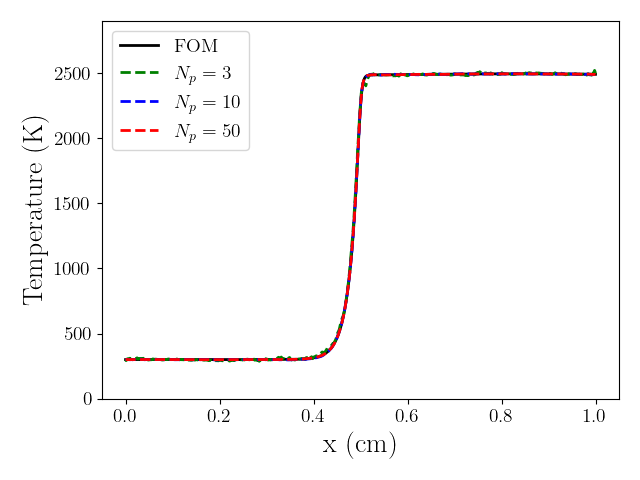
\includegraphics[width=0.99\linewidth]{Chapters/TransientFlame/Images/nonlinear/proj_temp_snaps.png}
    \end{minipage}
    \begin{minipage}{0.49\linewidth}
        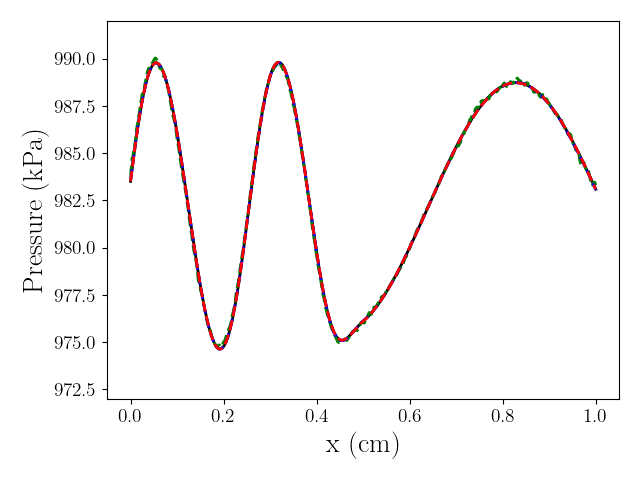
\includegraphics[width=0.99\linewidth]{Chapters/TransientFlame/Images/nonlinear/proj_press_snaps.png}
    \end{minipage}
    \caption{\label{fig:flameNonlinProj}Approximation of temperature (left) and pressure (right) fields on solution manifold, $f = 150$ kHz, $\timeVar = 250 \mu$s, various $\numPrimModes$.}
\end{figure}

The resulting autoencoders display exceptional accuracy in approximating the flame flow fields. Figure~\ref{fig:flameNonlinProj} shows the closest solution on the trial manifold (in the Euclidean norm) for temperature and pressure field snapshots. Even for $\numPrimModes = 3$, the representation is nearly perfect. Very close inspection reveals some low-amplitude noise, but larger latent space dimensions appear to entirely eliminate this. At first glance, this would appear to bode well for the resulting non-linear manifold PROMs.

\begin{figure}
    \begin{minipage}{0.49\linewidth}
        \includegraphics[width=0.99\linewidth]{example-image-a}
    \end{minipage}
    \begin{minipage}{0.49\linewidth}
        \includegraphics[width=0.99\linewidth]{example-image-a}
    \end{minipage}
    \caption{\label{fig:flameNonlinROM}Intrusive non-linear manifold MP-LSVT PROM snapshots, $\timeVar = XXX$, various $\numPrimModes$.}
\end{figure}

The same simulation configuration used for the linear subspace MP-LSVT PROMs is repeated here. Unfortunately, the autoencoder non-linear manifold PROMs also perform very poorly. In contrast to the over-smooth solutions generated by the linear trial spaces, the non-linear manifold PROMs suffer from excessive low-amplitude noise in the predicted solution. This is made apparent in Fig.~\ref{fig:flameNonlinROM}, revealing that the solution quickly devolves into meaningless noise where the approximate solution shown in Fig.~\ref{fig:flameNonlinProj} was so accurate. Ultimately, these non-linear PROMs suffer from an accumulation of error over a large number of time steps. These small errors appear to be amplified by the non-linear nature of the decoder: small deviations in the latent variables may lead to drastic changes in the predicted solution. Whereas linear trial space are relatively limited in their expressiveness, neural networks have the ability to generate both very accurate and very wrong solutions.

\begin{table}
	\centering
	\begin{tabular}{ lll }
	\toprule
	Model & Runtime (hours) & Cost (FOM runs)  \\
	\midrule
    Online FOM ($\times 1$) & 0.42 & 1 \\
    Training, $\numPrimModes = 3$ & 5.8 & 13.81 \\
    Training, $\numPrimModes = 10$ & 4.9 & 11.67 \\
    Training, $\numPrimModes = 50$ & 5.5 & 13.1 \\
    Online NLM PROM, $\numPrimModes = 3$ & 7.2 & 17.14 \\
	\bottomrule
	\end{tabular}
	\caption{\label{tab:caeCost}Relative offline/online computational costs for CAE PROMs. Non-increasing CAE training costs are due to early stopping.}
\end{table}

Not only is the accuracy of these non-linear manifolds PROMs disappointing, the cost to train and evaluate these models is exorbitant. Table~\ref{tab:caeCost} summarizes the cost of training and computing the neural network models, revealing that each step accounts for over ten times that of a single FOM simulation. The vast majority of the computational cost for the non-linear manifold PROM lies in calculating the Jacobian of the decoder, which relies on slow automatic differentiation procedures. Opposed to the simple analytical Jacobians possible for linear representations, it is difficult to justify the cost of this method given its experimental performance.

\section{Recurrent Neural Network ROMs}

A number of efforts have been undertaken in applying \textit{non-intrusive} approaches to reduced-order modeling. Such approaches do not require access to or even understanding of the underlying numerical solver, but only the outputs of the solver. Unlike PROMs which directly manipulate the governing equations, non-intrusive approaches are constructed wholly from data and evaluated independently from the numerical solver. Prominent examples include operator inference~\cite{Peherstorfer2016,Qian2020}, Koopman learning~\cite{Pan2021}, and a host of neural network approaches~\cite{Gonzalez2018,Xu2020,Maulik2020}. 

This work follows the method first formulated by Gonzalez and Balajewicz~\cite{Gonzalez2018}, which proposes the use of a long short-term memory (LSTM) network to model the evolution of the latent variables in time. The LSTM is a specific architecture of recurrent neural networks (RNNs), a form of neural network which performs auto-regressive predictions. That is, the network takes as input a series of past observations to make a prediction for the next step in the series, after which point that prediction is fed back into the network as input for the proceeding prediction, and so on. This design makes LSTMs ideal for time-series predictions, as in the case of reduced-order models for dynamical systems. Details on the mathematics of LSTMs (and RNNs more broadly) can be found in the review by Yu \textit{et al.}~\cite{Yu2019}. 

\begin{figure}
    \centering
    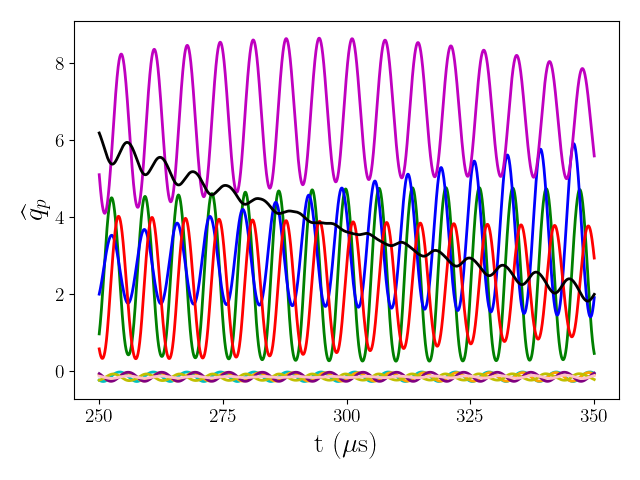
\includegraphics[width=0.6\linewidth]{Chapters/TransientFlame/Images/nonlinear/latent_vars.png}
    \caption{\label{fig:flameLatentVars}Encoded latent state trajectories, $f = 150$ kHz, $\numPrimModes = 10$.}
\end{figure}

For this work, two variants of LSTMs are trained: one trained using the modal coefficient trajectories associated with the linear trial space from Section~\ref{sec:flameLinear}, and one trained using the encoded latent variable trajectories associated with the autoencoder from Section~\ref{sec:flameNonlin}. This effectively compares the approaches of Maulik \textit{et al.}~\cite{Maulik2020} and Gonzalez and Balajewicz~\cite{Gonzalez2018}, respectively.

The LSTM training process is as follows. First, the training data is projected (for the POD representation) or encoded (for the CAE representation). Figure~\ref{fig:flameLatentVars} displays a representative trajectory of the latent variables for the autoencoder with $\numPrimModes = 10$. Then, standalone LSTM networks are trained using contiguous time windows of the training latent variable data. For this work, the LSTMs are constructed from two LSTM layers, followed by a single fully-connected layer that maps to the latent dimension $\numPrimModes$. The output size of both LSTM layers is 200, while the lookback window for the network inputs is 50 time steps. The LSTM layers are equipped with tanh activation functions, and the dense layer with a linear activation. The training parameters are the same as for the autoencoders. 

\begin{figure}
    \begin{minipage}{0.49\linewidth}
        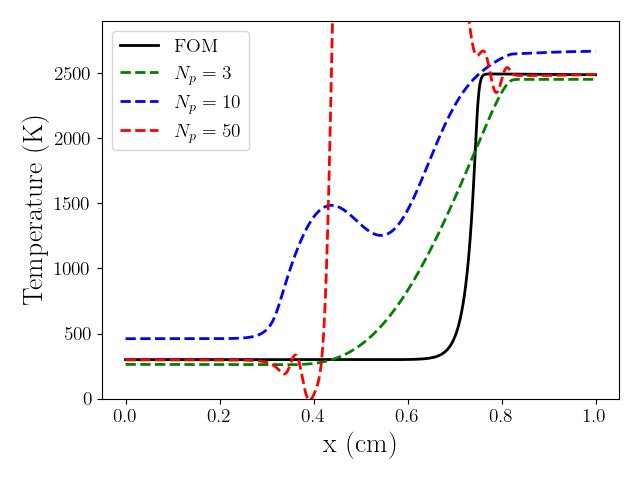
\includegraphics[width=0.99\linewidth]{Chapters/TransientFlame/Images/lstm/pod_rom_temp_snaps.png}
    \end{minipage}
    \begin{minipage}{0.49\linewidth}
        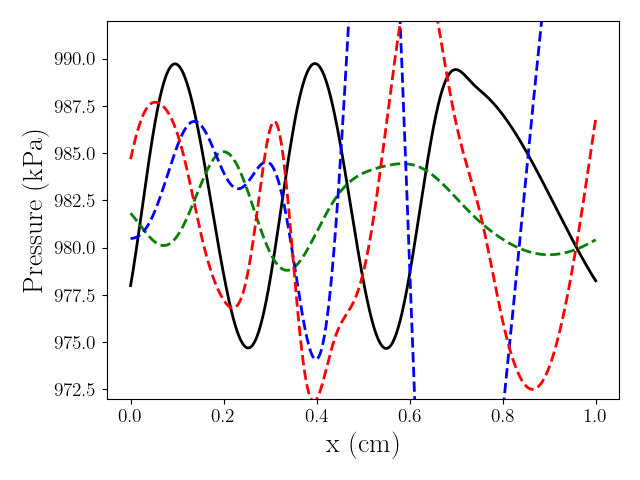
\includegraphics[width=0.99\linewidth]{Chapters/TransientFlame/Images/lstm/pod_rom_press_snaps.png}
    \end{minipage}
    \caption{\label{fig:flamePODLSTMFields}Online temperature (left) and pressure (right) field predictions for LSTMs trained with POD trajectories, $\timeVar = 500 \mu$s, $f = 131.25$ kHz, various $\numPrimModes$.}
\end{figure}

Evaluating these non-intrusive ROMs reveals stark contrasts in performance between the POD and CAE representations. Figure~\ref{fig:flamePODLSTMFields} displays predictions of the temperature and pressure fields near the end of the simulation window, for an unseen forcing frequency $f = 131.25$ kHz. As with the linear subspace PROMs, the ability of the POD modes to approximate the flow field remains extremely poor. At higher latent dimensions, the prediction appears to stagnate entirely. Although the pressure field retains an oscillatory nature, the predicted amplitude and frequency of the signal are wholly incorrect.

\begin{figure}
    \begin{minipage}{0.49\linewidth}
        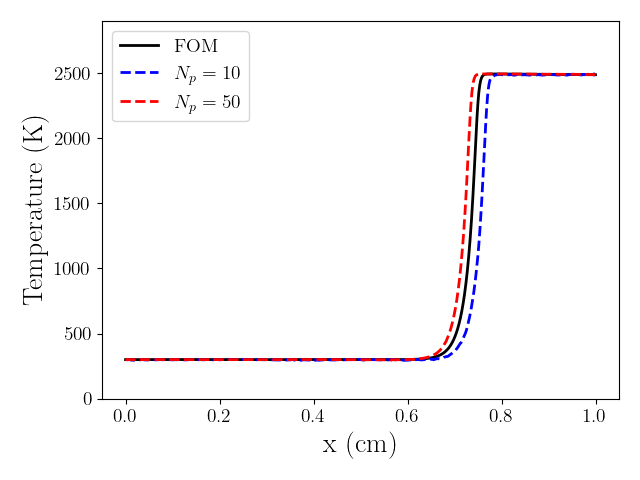
\includegraphics[width=0.99\linewidth]{Chapters/TransientFlame/Images/lstm/cae_rom_temp_snaps.png}
    \end{minipage}
    \begin{minipage}{0.49\linewidth}
        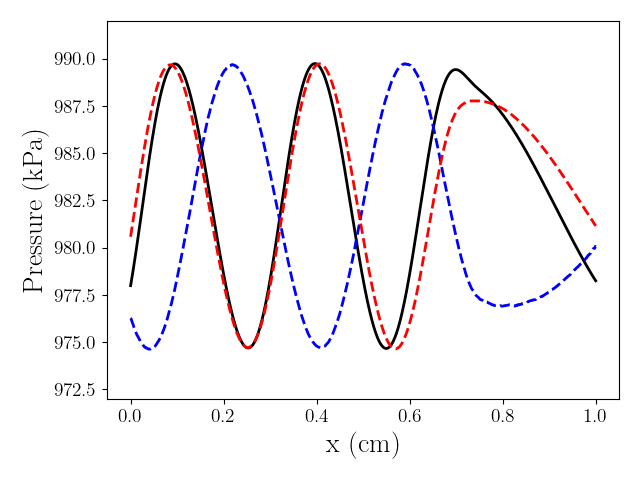
\includegraphics[width=0.99\linewidth]{Chapters/TransientFlame/Images/lstm/cae_rom_press_snaps.png}
    \end{minipage}
    \caption{\label{fig:flameCAELSTMFields}Online temperature (left) and pressure (right) field predictions for LSTMs trained with CAE trajectories, $\timeVar = 500 \mu$s, $f = 131.25$ kHz, various $\numPrimModes$. Note that $\numPrimModes = 3$ was unstable.}
\end{figure}

The LSTMs equipped with an autoencoder representation, on the other hand, perform exceptionally well. Figure~\ref{fig:flameCAELSTMFields} shows the same time instance as in Fig.~\ref{fig:flamePODLSTMFields}, but the long-term flow behavior is predicted very well. The temperature profile remains sharp and has progressed at similar speed as in the FOM, and the amplitude and frequency of the pressure signal appear to be preserved (albeit with some phase shift). However, it must be noted that the case for $\numPrimModes = 3$ was unstable, unlike that of the POD representation.

\begin{figure}
    \begin{minipage}{0.49\linewidth}
        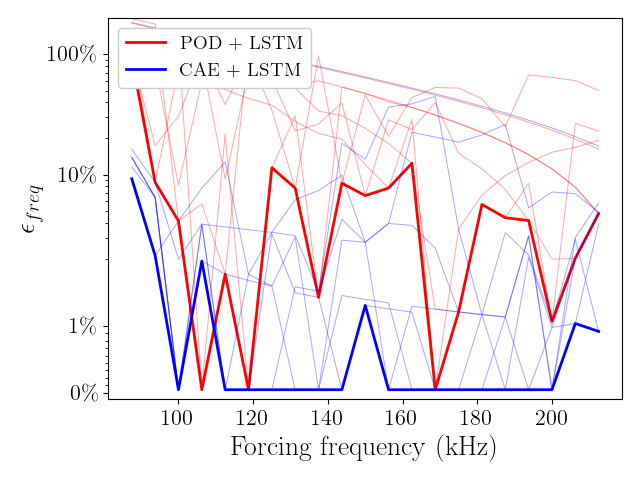
\includegraphics[width=0.99\linewidth]{Chapters/TransientFlame/Images/lstm/freq_err.png}
        \subcaption{Upstream $f$.}
    \end{minipage}
    \begin{minipage}{0.49\linewidth}
        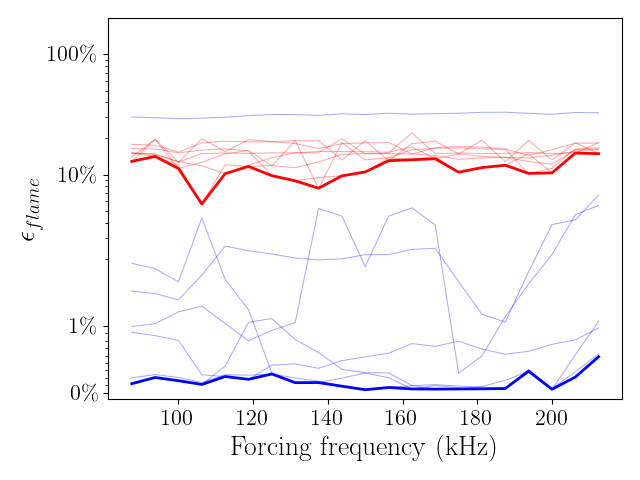
\includegraphics[width=0.99\linewidth]{Chapters/TransientFlame/Images/lstm/err_flame.png}
        \subcaption{Flame location.}
    \end{minipage}
    \caption{\label{fig:flameFreqFlameErr}Aggregate predictions of QoIs across all forcing frequencies, all $\numPrimModes$. The best predictions for each model are marked by a bold line.}
\end{figure}

Comparing these simulations quantitatively can be slightly challenging, as a minor phase shift in the predicted pressure field can result in enormous $\ell^2$-norm error measurements. Instead, two quantities of interest are measured: the predicted dominant frequency of the pressure signal at $x = 0.25$ cm (computed from the FFT of a point monitor, compared by amplitude), and the time-average accuracy of the flame location, as measured by the point of maximum heat release. Figure~\ref{fig:flameFreqFlameErr} summarizes the findings across all forcing frequencies and latent dimensions $\numPrimModes \in \{3, 5, 10, 20, 50, 100, 200\}$. The best predictions are connected by a bold line, while all others appear as translucent lines. Clearly, the LSTMs with a CAE representation are capable of predicting these QoIs with much higher fidelity than those with a POD representation. In fact, as hinted by the field plots in Fig.~\ref{fig:flamePODLSTMFields}, the frequency predictions of the the POD LSTM may be slightly misleading, as spurious frequencies of varying amplitudes may have been introduced.